% This file contains all homework from week 38
% use \section{<name>}  to create a section per homework assignment

\section[Homework 4]{Homework 4: XUTools}

XUTools manipulate files in terms of language-specific constucts, like C functions, IOS interface blocks and XML elements.


Traditional Unix Tools work on regular languages which don't work well with hierachical object models. Therefore the goal is to extend unix tools and the kind of languages they work on from regular languages to context-free languages.


XUTools presents eXtended Unix text-processing tool (XUTools) that enable extracting, counting and comparing in terms of language-specific constructs. The XUTools use a library of language grammars and xupath which is an xpath-like querying language to perform its operations. The following tools are considered the XUTools:

\begin{itemize}
	\item \textit{xugrep}
	\item \textit{xuwc}
	\item \textit{xudiff}
\end{itemize}

The goal is to extend more traditional unix tool into their extended form.

The eXtended Tools are dicussed in the ordered as shown in table~\ref{table:xutools}, below.\\

\begin{table}[h!]
\begin{center}
\begin{tabular}{ l | r }
	\hline
1.&xugrep\\ \hline
2.&xuwc\\ \hline
3.&xudiff\\
	\hline
\end{tabular}
\end{center}
\caption{XUTools}
\label{table:xutools}
\end{table}

\newpage

\subsection{xugrep}

Xugrep extracts text patterns in terms of higher-level-language constructs \cite{xutools01}.\\

\underline{Use cases for xugrep:} \\ \\

\textbf{Network Configuration Management}: Extract all interface blocks from a router configuration file that have applied a certain access list\\
\textbf{Developers}: Be able to grep for a function name as a function name\\
\textbf{Security Analyst}: grep the XML feed of how many times a specific entry occurs relative to another value\\

\textcolor{red}{The concept is shown in figure~\ref{fig:xugrep}.}\\

\begin{center}
        \begin{figure}[h!]
          \centering
                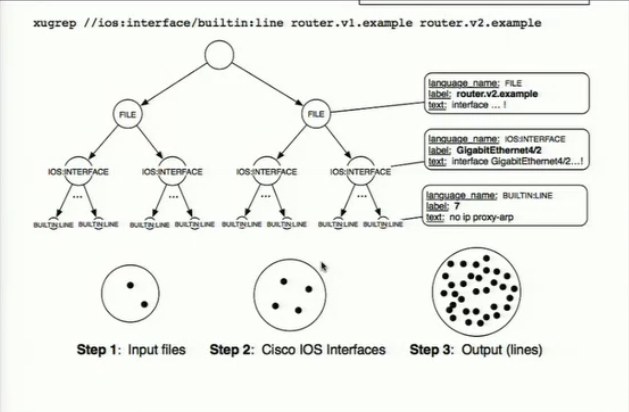
\includegraphics[scale=0.8]{xugrep}
          \caption{xugrep}
          \label{fig:xugrep}
        \end{figure}
\end{center}
\newpage

\subsection{xuwc}

Xuwc makes it possible to count text by understanding the structure for a specific language. So xuwc basically understands to language hierarchy in order to perform its job, which is counting \cite{xutools01}. \\

\underline{Use cases for xuwc:} \\ \\

\textbf{Network Configuration Management}: Perform easy and quick longitudinal studies on their own configuration data\\
\textbf{Developers}: Easily count the number of functions and lines per function\\
\textbf{Security Analysts}: Easily count the number of paragraphs per section or subsection of a policy and show the changes of by using the counting\\

\textcolor{red}{The concept is shown in figure~\ref{fig:xuwc}.}\\

\begin{center}
        \begin{figure}[h!]
          \centering
                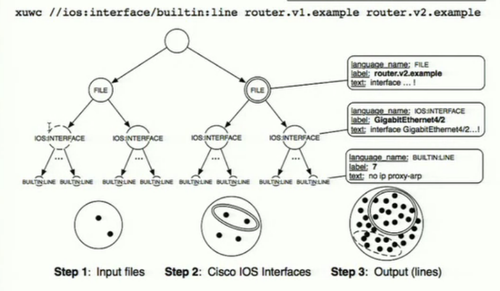
\includegraphics[scale=0.8]{xuwc}
          \caption{xuwc}
          \label{fig:xuwc}
        \end{figure}
\end{center}
\newpage

\subsection{xudiff}

Xudiff compares two files in terms of higher-level-language constructs \cite{xutools01}.\\

\underline{Use cases for xudiff:} \\ \\

\textbf{Network Configuration Management}: Capture the changes of configuration files to have a good overview of what changed\\
\textbf{Developers}: Capture the changes of a functions different levels\\
\textbf{Security Analyst}: Capture the changes of a section and subsection rather than per line\\

\textcolor{red}{The concept is shown in figure~\ref{fig:xudiff}.}\\

\begin{center}
        \begin{figure}[h!]
          \centering
                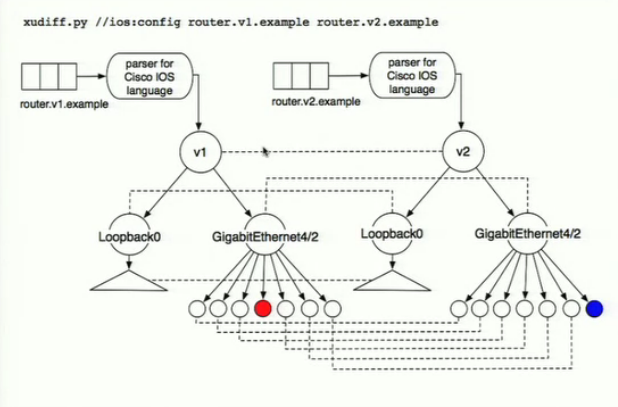
\includegraphics[scale=0.8]{xudiff}
          \caption{xudiff}
          \label{fig:xudiff}
        \end{figure}
\end{center}

